% Compile with:
% pdflatex main.tex
% bibtex main
% pdflatex main.tex
% pdflatex main.tex
\documentclass[letterpaper]{article}
\usepackage[submission]{aaai2027}
\usepackage[hyphens]{url}
\usepackage{graphicx}
\urlstyle{rm}
\def\UrlFont{\rm}
\usepackage{natbib}
\usepackage{caption}
\usepackage{placeins}
\frenchspacing

\usepackage{amsmath}
\usepackage{amssymb}
\usepackage{amsthm}
\usepackage{mathtools}
\usepackage{booktabs}

\setcounter{dbltopnumber}{3}
\renewcommand{\dbltopfraction}{0.95}
\renewcommand{\textfraction}{0.04}
\renewcommand{\dblfloatpagefraction}{0.90}

\pdfinfo{
/TemplateVersion (2027.1)
}

\newtheorem{definition}{Definition}
\newtheorem{theorem}{Theorem}
\newtheorem{proposition}{Proposition}

\newcommand{\system}{\textsc{AlgoTutorGen}}
\newcommand{\machineok}{\textsc{Machine OK}}
\newcommand{\traceir}{\textsc{SemanticTrace}}
\newcommand{\scenegraph}{\textsc{SceneGraph}}
\newcommand{\runtime}{\textsc{Web Runtime}}
\newcommand{\ssv}{\textsc{SSV}}
\newcommand{\pvcr}{\textsc{PVCR}}
\newcommand{\localresume}{\textsc{Local Resume}}
\newcommand{\globalrestart}{\textsc{Global Restart}}
\newcommand{\benchmarkname}{\textsc{AlgoTutorGen-Bench}}
\newcommand{\dbr}{\textsc{Direct-BrowserRepair (max 5)}}
\newcommand{\htmlcure}{\textsc{HTMLCure (strict)}}
\newcommand{\vtllm}{\textsc{VerifiedTrace-to-LLM-HTML}}

\setcounter{secnumdepth}{2}

\begin{document}

\title{AlgoTutorGen: Service-Compositional Semantic Tracing for Reliable and Auditable Interactive Algorithm Tutors}
\author{Anonymous Submission}
\affiliations{}

\maketitle

\begin{abstract}
LLMs can display the expected answer in an algorithm tutor yet fail to
produce a reliable interactive system. We introduce \system{}, which
establishes semantic ownership before presentation. One instrumented
solver over reusable state services jointly produces the answer, typed
events, per-step service snapshots, and runtime-captured source
callsites.
\emph{Semantic Synthesis and Verification} (\ssv{}) validates this
single-execution record and compiles a fixed-shell tutor;
\emph{Post-Verification Creative Rendering} (\pvcr{}) may redesign only
the central stage, with Verified-View fallback. On 200 tasks from 23
algorithm families, \system{} and Direct HTML both display the expected
answer on 200/200 pages, but satisfy the complete browser-level tutor
contract on 198/200 and 98/200 pages, respectively. The gap persists
across three additional LLMs and 40 held-out tasks. All 1,292 audited
runs pass the mechanical execution-to-trace checks; a blinded
source-to-trace audit finds 59/60 tasks trace-perfect and no confirmed
critical semantic error. Projection and randomized-interaction audits
find no tested preservation or noninterference violation. \pvcr{}
produces 200/200 layout-valid Creative Views and ranks first in both
frozen vision-language-model (VLM) evaluation and its human-calibration
subset. Together, these results support reliable and auditable
construction of interactive algorithm tutors.
\end{abstract}

\section{Introduction}
\label{sec:introduction}

LLMs increasingly generate executable visual artifacts, but visual
fidelity, successful compilation, and genuine interaction remain
distinct properties
\citep{si2025design2code,lu2025webgenbench,dai2026iwebgenbench}.
This distinction is critical for interactive algorithm tutors, which
must synchronize intermediate state, navigation, learner feedback,
hints, answer reveal, and learning logs without allowing teaching
actions to corrupt algorithmic facts. In our benchmark, Direct HTML and
\system{} both display the expected answer on 200/200 tasks, yet only
98 and 198 pages, respectively, satisfy the complete nine-part
browser-level \machineok{} contract.

To make these obligations measurable, \benchmarkname{} represents each
task as an executable bundle of concrete inputs, semantic trace checks,
required views, learner-interaction tasks, and assessment checks. This
benchmark distinguishes an answer-bearing page from a tutor that remains
behaviorally complete under browser execution.

Free-form generation assigns these obligations to the same mutable
page. We call this coupling \emph{constraint entanglement}:
independently authored state and visual updates can diverge, while
algorithm facts, runtime behavior, pedagogy, and presentation remain
writable through the same downstream artifact. Existing
educational-media, website-generation,
browser-repair, and trace-first systems address parts of this problem
\citep{ji2025eduvisagent,chen2025code2video,
lu2025webgenagent,wu2026htmlcure,
anonymous-etal-2026-algogen,tang2026vividoc}, but do not jointly
establish a canonical algorithm state and owners for the remaining
tutor behavior. Figure~\ref{fig:paradigms} contrasts these ownership
patterns.

\begin{figure*}[t]
\centering
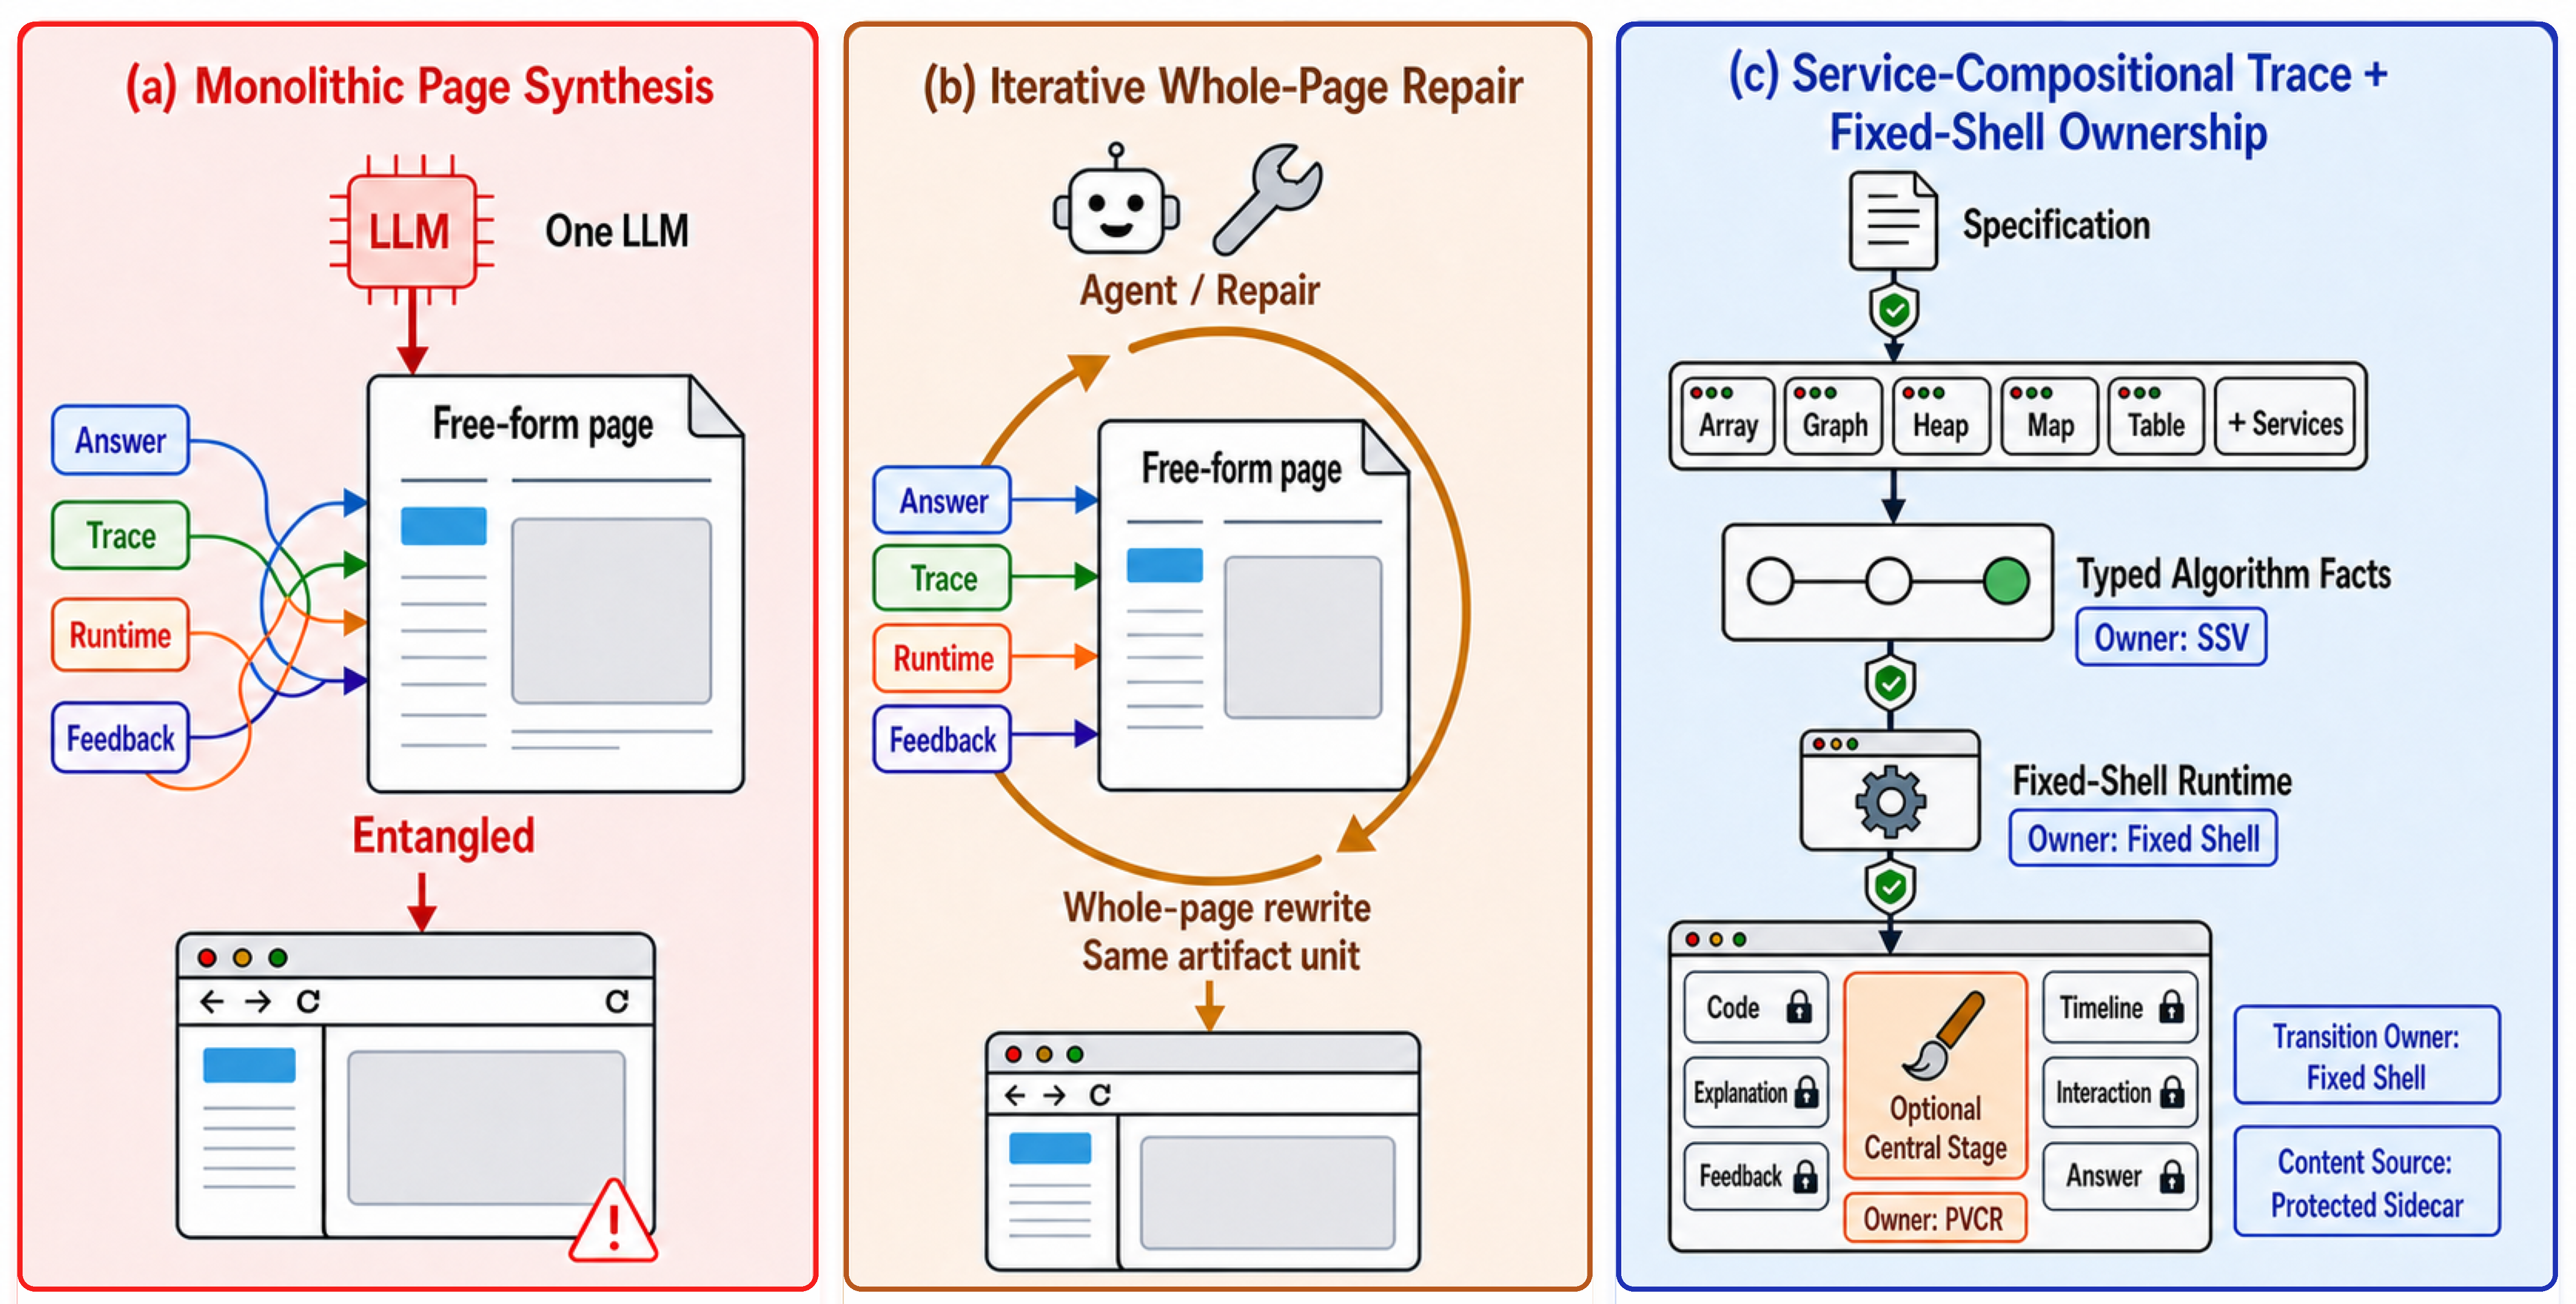
\includegraphics[width=0.90\textwidth]{figures/figure1-service-compositional-fixed-shell-candidate-20260726-tight.png}
\caption{Comparison of monolithic synthesis, whole-page repair, and
\system{}. \ssv{} owns semantic facts, the fixed shell owns runtime and
teaching transitions, and \pvcr{} owns only central-stage presentation.}
\label{fig:paradigms}
\end{figure*}

\system{} establishes \emph{semantic ownership before presentation}.
The model writes ordinary Python control flow over reusable state
services. One instrumented execution computes the answer while service
mutations atomically update represented state and emit typed events;
the same run also records per-step service snapshots and
runtime-captured source callsites. \ssv{} validates this bound record
and any available oracle,
deterministically compiles \scenegraph{} frames, and exports a
fixed-shell Verified View.

The fixed shell owns navigation, submissions, hints, answer reveal,
feedback transitions, and learning logs; generated pedagogical content
may interpret verified facts but, under the enforced interfaces, is not
permitted to rewrite them. After semantic
release, \pvcr{} may generate scoped assets only for the central stage.
Sanitization and browser/layout checks accept a Creative View or return
the Verified View. Open-ended visual generation is therefore placed
behind the semantic boundary.

Prior trace-first systems such as ALGOGEN separate generated tracking
from deterministic rendering~\citep{anonymous-etal-2026-algogen}.
ALGOGEN-style trackers update execution state and emit visualization
operations as separate model-authored actions. \system{} instead couples
supported state mutation to typed event emission and gives the fixed shell
ownership of the complete tutor interaction; our paired same-shell
separated-trace control makes this interface change experimentally
identifiable. Each check is applied at the earliest representation
where its corresponding defect becomes observable. Execution and oracle
checks precede semantic release, scene checks precede browser export,
and generated teaching or presentation is integrated only after the
protected record exists. A downstream component may reject an upstream
artifact, but under the enforced interfaces it cannot silently redefine
an accepted algorithm fact.

Across three additional LLMs and a 40-task held-out set, the reliability
advantage persists. Full-benchmark execution-record, source-to-trace,
projection, mutation, determinism, randomized-browser, service-reuse,
and visual-calibration audits test the proposed boundaries. The main
contributions are:
\begin{itemize}
    \item \textbf{Execution-bound service-compositional tracing.}
    Supported state mutations atomically emit typed semantic events
    within one instrumented solver execution that binds the answer,
    events, snapshots, and runtime-captured source callsites.
    \item \textbf{Protected interactive-tutor construction.}
    A deterministic fixed shell owns navigation, feedback, hints, answer
    reveal, and learning logs; generated pedagogy and central-stage
    rendering consume released facts without redefining them.
    \item \textbf{Mechanism-level and executable evidence.}
    \benchmarkname{} spans 200 tasks, 646 inputs, and 23 algorithm
    families, with executable semantic, visual, and interaction checks.
    \system{} achieves 198/200 complete browser reliability versus
    98/200 for Direct HTML; a same-shell comparison with an
    ALGOGEN-style separated-trace interface improves Machine OK from
    162/200 to 183/200, isolating the value of atomic state/event
    ownership beyond visible-answer or screenshot quality.
\end{itemize}

\begin{figure*}[t]
\centering
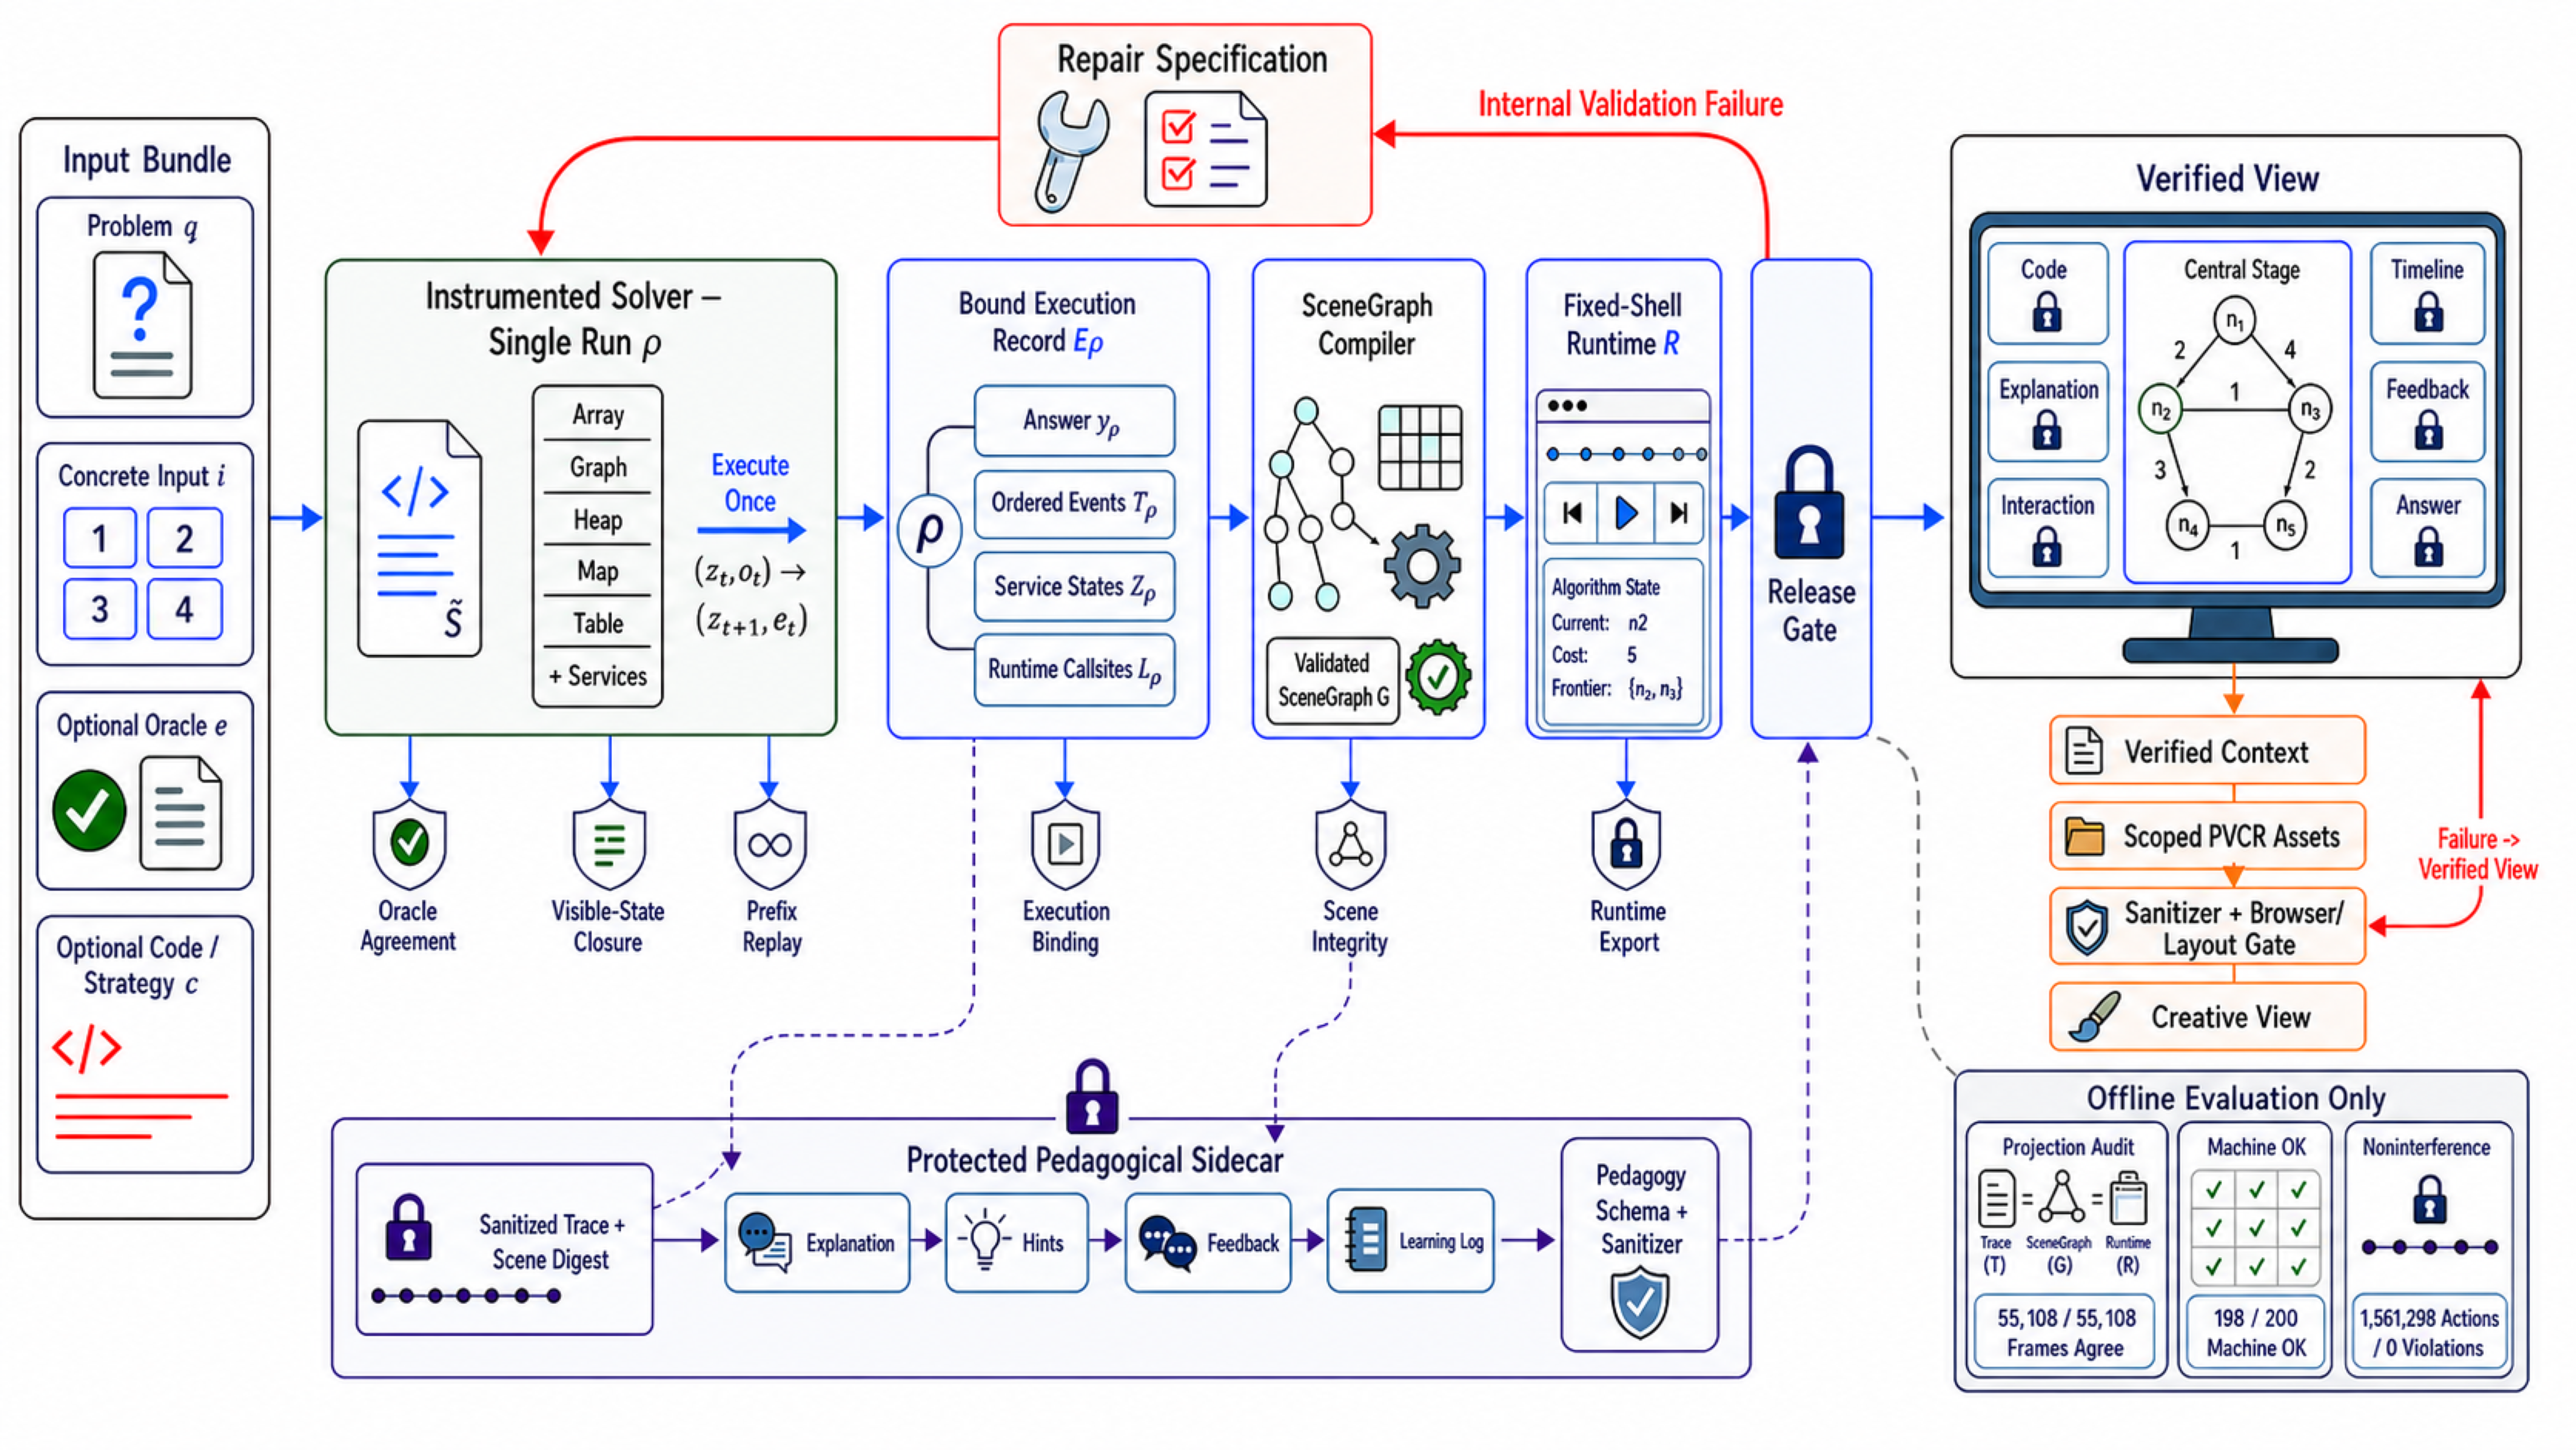
\includegraphics[width=0.94\textwidth]{figures/figure2-single-execution-ssv-pvcr-candidate-20260725.png}
\caption{\system{} architecture. One instrumented solver run binds the
answer, events, snapshots, and callsites. The protected sidecar cannot
own algorithm state; \pvcr{} contributes only central-stage assets with
Verified-View fallback, while \machineok{} and noninterference remain
offline audits.}
\label{fig:architecture}
\end{figure*}

\section{Related Work}
\label{sec:related_work}

\paragraph{Algorithm Visualization and Educational Generation.}
Classical systems provide curated execution views, exercises, and
reusable visualization libraries
\citep{Malmi2004TRAKLA2,Guo2013PythonTutor,
Karavirta2013JSAV,Shaffer2011OpenDSA,Halim2015VisuAlgo,Naps2005JHAVE},
but rely primarily on human-authored algorithms or templates.
These systems establish the value of synchronized execution views,
automatic assessment, and reusable interaction components. Generative
systems broaden the authoring process: EduVisAgent coordinates
instructional planning and visualization agents, while Code2Video
combines executable code with planner--coder--critic collaboration
\citep{ji2025eduvisagent,chen2025code2video}. Their primary artifact is
a pedagogically organized visualization or video, rather than a
self-contained generated browser tutor whose algorithm state,
navigation, bidirectional feedback, hint and answer behavior, and
learning state must jointly pass an executable contract. Prior
evaluations likewise treat learner engagement and learning outcomes as
distinct from visualization design
\citep{Naps2003Engagement,Hundhausen2002MetaStudy}.

\paragraph{Interactive Web Generation and Repair.}
Design2Code, WebGen-Bench, and I-WebGenBench distinguish visual
reproduction, build success, functional behavior, and event-driven
interaction
\citep{si2025design2code,lu2025webgenbench,dai2026iwebgenbench}.
WebGen-Agent incorporates screenshot and GUI-agent feedback into
iterative generation and selection, while HTMLCure executes pages
across browser states and uses trajectory-derived evidence to repair
state-dependent failures
\citep{lu2025webgenagent,wu2026htmlcure}. These systems substantially
advance functional website generation, but their generation or
revision unit remains the website or HTML artifact as a whole.
\system{} instead establishes an upstream canonical algorithm record
and gives different owners to semantic facts, shell behavior,
pedagogical content, and optional presentation. A later presentation
or feedback repair is therefore not permitted, under these interfaces,
to redefine an accepted algorithm fact.

\paragraph{Structured Traces and Executable Assurance.}
ALGOGEN separates generated tracking from deterministic rendering, and
ViviDoc places a structured document representation before interactive
code generation
\citep{anonymous-etal-2026-algogen,tang2026vividoc}. In ALGOGEN, an
LLM-generated tracker emits Visualization Trace Algebra operations and
a deterministic renderer combines the trace with a rendering language;
ViviDoc decomposes an interactive document into state, rendering,
transition, and constraint components before code generation. These
works motivate placing a structured representation before open-ended
presentation.

\system{} changes both the generated interface and the released
artifact. Unlike ALGOGEN, reusable state services jointly update
represented state and emit typed events, binding the answer, events,
snapshots, and runtime-captured callsites to one execution without a
second model-authored trace path. Unlike general interactive-document
generation, the fixed shell owns navigation, feedback, hints, answer
reveal, learning logs, and protected algorithm state. Specification-
guided synthesis, semantics-preserving compilation, noninterference,
and property-based testing motivate its explicit contracts and audits
\citep{SolarLezama2006Sketch,Polikarpova2016Synquid,
Gulwani2017ProgramSynthesis,Leroy2009CompCert,
Goguen1982Noninterference,Claessen2000QuickCheck,
Segura2016Metamorphic}.

\section{Method}
\label{sec:method}

\subsection{Task Formulation and Pipeline Overview}
\label{sec:method_overview}

For input \(x=(q,i,e,c)\), consisting of a problem, concrete instance,
optional oracle, and optional reference code or strategy, \system{}
constructs a self-contained tutor through
\[
\begin{aligned}
\widetilde S
&\xrightarrow{\operatorname{execute}_{\rho}}
E_{\rho}=(y_{\rho},T_{\rho},Z_{\rho},L_{\rho})
   \xrightarrow{\operatorname{compile}} G,\\
G &\xrightarrow{\operatorname{export}(\bar{P},R)} W_V
   \xrightarrow{\operatorname{PVCR}} W_C.
\end{aligned}
\]
\(\widetilde S\) is one instrumented solver executed under identifier
\(\rho\). Its bound record contains the answer \(y_\rho\), typed events
\(T_\rho\), per-step service snapshots \(Z_\rho\), and runtime-captured
source callsites \(L_\rho\). Project code compiles \(T_\rho\) into
\scenegraph{} frames \(G\) and exports a fixed-shell Verified View
\(W_V\) with sanitized pedagogy \(\bar P\) and runtime \(R\).
\pvcr{} optionally returns a Creative View \(W_C\). Online release
checks execution binding, oracle agreement, trace admissibility, scene
integrity, and runtime export; stronger feedback and noninterference
checks remain offline audits. Figure~\ref{fig:architecture} summarizes
these asymmetric ownership boundaries.

Ownership is intentionally asymmetric. The model generates
\(\widetilde S\), pedagogical content before sanitization, and optional
\pvcr{} assets. It does not regenerate algorithm state at the scene or
browser stage. A downstream owner may reject an upstream artifact, but
under the enforced interfaces is not permitted to silently replace a
fact already released by that owner.

For an SSV artifact \(A=(\widetilde S,E_\rho,G,\bar P,R)\), the online
release boundary is
\[
\Phi_{\mathrm{release}}
=
\Phi_{\mathrm{execution}}
\land\Phi_{\mathrm{result}}
\land\Phi_{\mathrm{trace}}
\land\Phi_{\mathrm{scene}}
\land\Phi_{\mathrm{runtime}}.
\]
The terms check same-execution binding and callsites, available-oracle
agreement, trace admissibility, scene integrity, and fixed-shell export.
Feedback quality and pedagogical noninterference are stronger offline
evaluation obligations, rather than conditions claimed to be
mechanically established for every future page.

\subsection{Service-Compositional Trace Synthesis}
\label{sec:service_trace}

\paragraph{Atomic state and event ownership.}
Rather than generating separate algorithm-state and visual-update
commands, the model writes ordinary Python over reusable
\textsc{TraceSession} services. The current catalog contains 21
services for indexed and associative state, ordered containers, graphs,
trees, linked structures, and range data structures. For service
\(v_j\), operation \(o_t\) atomically couples state transition and
event emission:
\[
\bigl(z_{t+1}^{(j)},\,e_t\bigr)
=
\operatorname{step}_{v_j,o_t}
\bigl(z_t^{(j)};\rho,\ell_t\bigr),
\qquad
T=(e_0,\ldots,e_n).
\label{eq:service_step}
\]
Events carry stable object identifiers, operation type, before/after
values, dependencies, and \(\rho\); runtime instrumentation captures
\(\ell_t\), which is supplied by instrumentation rather than model
output. A Dijkstra solver, for
example, composes graph, map, and heap services. Updating a tentative
distance or pushing a frontier item changes represented state and emits
the corresponding event, from which presentation is derived. Stable
identifiers let the same entity be followed across trace, scene, and
runtime states without a second generated redraw command.
A paired ablation contrasts this atomic interface with a
decoupled-claim variant under the same downstream validators, compiler,
and fixed shell.

\paragraph{Specification and repair boundary.}
The model receives the problem, concrete input, optional oracle, and
documented service interface, and returns one instrumented solver. The
same run commits the answer and exports its trace, snapshots, and
callsites. Ordinary local variables are permitted, but every canonical
fact released to the tutor must originate from service state or an
explicit checked event. The final answer is not copied from a second
generated function.

The generation interface does not permit solvers to emit HTML, CSS, DOM
handlers, renderer coordinates, or browser controls. Before execution,
the system checks
the specification schema, required signatures, permitted imports, and
documented service methods; the candidate then runs in a bounded child
process. Schema, sandbox, execution, and post-execution failures return
structured diagnostics for a bounded full-specification repair. The
model receives the previous complete specification and validator
diagnostics rather than an unconstrained self-critique; unrepaired
candidates are rejected. The service catalog, signatures, prompts, and
repair protocol appear in the supplement.

\subsection{Semantic Synthesis and Verified Tutor Construction}
\label{sec:ssv_construction}

\paragraph{Execution-record validation.}
Validators check common-run identifiers and callsites, typed operations
and continuous transitions, object references, visible-state closure,
prefix replay against every recorded service state, final-state
equality, and agreement with any available oracle. A frame may contain
values, marks, pointers, graph edges, containers, source references,
and the answer, but no CSS, DOM nodes, or handlers. These checks
establish fidelity to the instrumented execution for service-mediated
state. Oracles, reference tests, and the sampled human audit
independently evaluate algorithm correctness.

\paragraph{Deterministic compilation and fixed shell.}
The deterministic compiler produces
\[
G=\operatorname{Compile}(T)=(G_0,\ldots,G_n).
\]
Each accepted event induces a \scenegraph{} frame while preserving
object identities and references. Service roles constrain eligible
bindings: indexed state maps to arrays or tables, graph services to
nodes and edges, maps to key--value views, and ordered containers to
frontier or stack views. Optional deterministic hints may choose among
eligible layouts but are not permitted to redefine trace state. The
scene gate checks
nonempty output, supported objects, valid bindings, and cross-frame
identity.

The shared runtime exports only validated frames into \(W_V\) and owns
navigation, submissions, hints, answer reveal, feedback transitions,
and learning logs. The browser release gate checks self-containment,
loading, required controls, and exported state; complete behavioral and
randomized-action tests remain offline. Validation is therefore
boundary-specific: specification checks precede execution, replay and
oracle checks follow materialization, reference checks follow scene
compilation, and browser checks follow export.

\begin{figure*}[t]
\centering
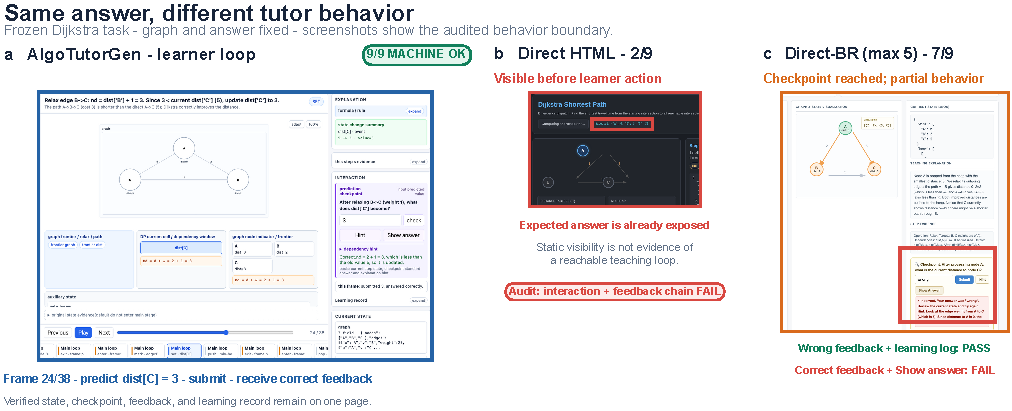
\includegraphics[width=0.90\textwidth]{figures/qualitative_dijkstra_main.pdf}
\caption{Frozen Dijkstra case with the same graph and expected answer.
Panel (a) completes predict--submit--correct feedback; panel (b) exposes
the answer before learner action; panel (c) reaches a checkpoint but fails
correct-feedback and answer-reveal checks. The full five-method matrix is
in the supplement.}
\label{fig:case-dijkstra}
\end{figure*}

\subsection{Read-Only Pedagogy and Scoped Rendering}
\label{sec:pedagogy_pvcr}

\paragraph{Read-only pedagogy.}
A sanitized digest of validated events and frames may support
explanations, hints, mistake descriptions, and prediction checkpoints.
This read-only pedagogical sidecar is represented in the artifact as
the sanitized overlay \(\bar P\).
It exposes selected operations, affected objects, before/after values,
dependencies, and source references, but grants no trace ownership. The
overlay may interpret verified facts and update pedagogical state, while
fields that attempt to modify algorithm state, answer, dependencies,
event order, or protected references are removed or rejected. The fixed
shell, not generated teaching code, executes state-changing teaching
behavior. Consequently, pedagogical content can vary across tasks while
the execution of navigation, prediction submission, hint and answer
reveal, feedback updates, and learning-log writes remains shared.

\paragraph{Scoped creative rendering.}
After \(W_V\) passes release, \pvcr{} receives read-only verified
context containing the problem, concrete input, verified result,
release summary, state keys, and selected verified frames. It may return
only central-stage styles, a template, and a frame-consuming renderer.
Accepted \pvcr{} assets are restricted from replacing shell-owned
panels, redefining navigation, or writing protected fields.
Sanitization and browser/layout checks guard
integration. One bounded presentation-only repair is permitted;
accepted assets yield \(W_C\), otherwise the system releases \(W_V\).
Thus creative generation cannot reduce Verified-View availability. The
complete asset and fallback contract is in the supplement.

\subsection{Conditional Design Properties}
\label{sec:design_properties}

The following implications state the intended boundaries; full
definitions and proofs appear in the supplement.

\smallskip\noindent
\textbf{Property 1 (Trace fidelity).}
Let \(z_t\) be the complete service-mediated state before event \(e_t\).
If every released canonical fact is service-mediated or explicitly
checked, service mutation and event emission are atomic, source
callsites are runtime-captured, and out-of-service mutations are
rejected, then for
every event prefix \(k\),
\[
\operatorname{Replay}(z_0,e_{<k})=z_k,
\]
and the answer, events, snapshots, and callsites belong to execution
\(\rho\). This establishes fidelity to the instrumented execution, not
that the solver implements the intended algorithm.

\smallskip\noindent
\textbf{Property 2 (Semantic preservation).}
Let \(\mathcal A\) contain representation-independent algorithm facts:
stable identifiers, values, marks, pointers, edges, containers, step,
and answer, excluding layout, CSS, explanations, hints, and logs.
Define canonical projections
\[
\alpha_T:T_t\!\to\!\mathcal A,\qquad
\alpha_G:G_t\!\to\!\mathcal A,\qquad
\alpha_R:R_t\!\to\!\mathcal A.
\]
If \(\alpha_T(T_t)=\alpha_G(G_t)\) and
\(\alpha_G(G_t)=\alpha_R(R_t)\) for every corresponding frame, then
\(\alpha_T(T_t)=\alpha_R(R_t)\); the rendered answer equals the answer
committed by the same execution record. Agreement of that answer with
an available oracle remains a separate premise.

\smallskip\noindent
\textbf{Property 3 (Pedagogical noninterference).}
Write runtime state as protected algorithm state \(a\) and pedagogical
state \(p\), so \(\sigma=(a,p)\). If every pure teaching action \(u\)
satisfies
\[
\delta_u(a,p)=(a,p')
\]
and navigation selects only algorithm states released by validated
traces, then teaching-only sequences preserve their initial \(a\),
while mixed sequences keep \(a\) within the released set. Projection,
mutation, preserving-transformation, determinism, and
randomized-browser audits test these premises on the evaluated artifacts
and operators. Full statements and proofs appear in the supplement.

\begin{table*}[t]
\centering
\small
\setlength{\tabcolsep}{6pt}
\begin{tabular}{lrrr}
\toprule
\multicolumn{4}{c}{\textit{A. Primary final \machineok{} outcomes}}\\
Method & Pass & Method & Pass \\
\midrule
\system{} Verified View & \textbf{198/200} & Direct HTML & 98/200 \\
WebGen-Agent & 45/200 & \htmlcure{} & 40/200 \\
\dbr{} & 120/200 & & \\
\midrule
\multicolumn{4}{c}{\textit{B. Paired model and held-out robustness}}\\
Condition & \system{} & Direct & Difference \\
\midrule
DeepSeek-V4-Pro & 198/200 & 98/200 & +50.0 pp \\
DeepSeek-V4-Flash & 200/200 & 118/200 & +41.0 pp \\
GLM-5.2 & 196/200 & 35/200 & +80.5 pp \\
Kimi-K2.5 & 194/200 & 87/200 & +53.5 pp \\
Held-out, 15 families & 39/40 & 18/40 & +52.5 pp \\
\bottomrule
\end{tabular}
\caption{Executable reliability under frozen policies (A) and paired
model and held-out robustness (B).}
\label{tab:reliability-main}
\end{table*}

\section{Experimental Setup}
\label{sec:setup}

\benchmarkname{} contains 200 tasks from 23 algorithm families and 646
concrete inputs. Each task bundles problem metadata, concrete instances,
executable solver/tracker/verifier programs, required views, learner
interactions, and assessment checks; the full benchmark overview appears
in the supplement.
Main paired evaluation uses one input per task; 446 additional inputs
support replay, and 40 new cases from 15 supported families form the
held-out set. The primary \system{} and Direct HTML
runs use DeepSeek-V4-Pro; frozen robustness runs use
DeepSeek-V4-Flash, GLM-5.2, and Kimi-K2.5. WebGen-Agent,
\htmlcure{}, and \dbr{} are task-adapted baselines
audited by the same final browser protocol.

Direct generates one self-contained page from the same task and
expected answer; \system{} may use two candidates and two repair rounds.
\dbr{} applies adaptive early-stopping and best-so-far whole-page repair
to a separately frozen 200-page Direct set, using at most five repair
calls per task. The primary comparison evaluates final artifacts under
frozen generation-and-repair policies; token-matched reliability and
full cost accounting appear in the supplement.

\machineok{} conjoins page load, visible-answer match, reachable
interaction, correct and wrong feedback, hint, answer reveal, learning
log, and protected-answer stability. Paired outcomes use exact
two-sided McNemar tests and task-level bootstrap intervals. The audit
covers two accepted variants of all tasks over 646 inputs (400
programs; 1,292 runs). Mechanical and negative-fault audits validate
execution binding, source coverage, replay, final-state equality, oracle
agreement, visible-state closure, and deterministic replay; complete
audit definitions and statistical boundaries are in the supplement.

Two algorithmically trained reviewers independently label both accepted
variants of 60 stratified tasks spanning all 23 families (120 traces;
3,883 events). Reviewers are blinded to method identity, automatic
outcomes, and each other's labels. Their event labels cover source
alignment, state transition, algorithmic operation, and explanation
consistency. A method-hidden 1--5 visual rubric is calibrated on 150
pages from 30 tasks. Complete reviewer definitions are in the
supplement.

\section{Results}
\label{sec:results}

\subsection{Executable Reliability}
Table~\ref{tab:reliability-main} shows 198/200 \machineok{} pages for
\system{} versus 98/200 for Direct, a paired difference of \(+50.0\)
points (95\% CI [43.0, 57.0], McNemar
\(p=4.06\times10^{-29}\)). Both expose the expected answer on 200/200
pages, localizing the gap to interaction and teaching behavior. Direct
failures arise mainly after loading, at interaction and bidirectional
feedback boundaries: cumulative survival falls from 94.0\% after load
to 74.5\% after reachable interaction, 54.0\% after bidirectional
feedback, and 49.0\% after the complete contract, whereas \system{}
remains at 99.0\%. \dbr{} reaches 120/200 \machineok{} pages under
adaptive early stopping and best-so-far selection, remaining 39.0
percentage points below \system{}. At matched total-token cost
(approximately 84.3k per task), the 198/200 versus 120/200 gap remains
(supplement).
Figure~\ref{fig:case-dijkstra} makes this distinction concrete on one
frozen Dijkstra task: all methods expose the same expected answer, while
only the \system{} page satisfies the complete nine-part tutor contract.

On 50-task ablations, the
full chain passes 49/50, versus 1/50 for Direct-to-SceneGraph and 0/50
for \vtllm{}. On these 50-task ablations, neither a fixed renderer
without executable trace construction nor a verified trace followed by
unconstrained page generation reproduces the connected chain.

\paragraph{Atomic-service ablation.}
In a separate paired Full-200 run, Atomic-service and the
ALGOGEN-style separated-trace condition use the same tasks, model,
generation policy, validators, compiler, and fixed shell. In the
separated-trace condition, ordinary Python state is updated first and
the model separately emits the corresponding event claim; no helper
couples the two operations. Atomic-service increases \machineok{} from
162/200 to 183/200 (\(+10.5\) points; 95\% CI [3.5, 17.0]; McNemar
\(p=0.00460\)) and generation pass from 164/200 to 187/200
(\(+11.5\) points; \(p=0.00109\)). All 152 paired auditable records
pass the same execution-consistency checks in both conditions, showing
that atomic state/event ownership improves valid-artifact yield under an
unchanged downstream validation standard.

\subsection{Execution and Source-to-Trace Fidelity}
All 1,292 instrumented runs pass the mechanical execution-record audit,
and the validator rejects 9,044/9,044 injected corruptions while
accepting 1,292/1,292 preserving controls. The blinded audit finds
59/60 tasks trace-perfect across both variants (98.3\%; Wilson 95\% CI
[91.1, 99.7]) and no confirmed critical semantic error; all 3,883
labeled state transitions and algorithmic operations are judged correct.
Of 3,880 source-verifiable events, 3,878 point to the exact or adjacent
line, while the other two remain aligned with the same logical statement
block. Both prespecified reviewer-agreement measures obtain Cohen's
\(\kappa=1.000\). An oracle-backed audit also rejects 60/60
wrong-but-self-consistent solver executions spanning all 23 families
(supplement).

\subsection{Semantic Preservation and State Isolation}
Across 294 artifacts, all 55,108 evaluated trace--scene--runtime frames
agree under canonical projection; 2,198/2,198 semantic mutations are
rejected and 392/392 preserving transformations accepted. The frame
total comprises 9,421 main, 4,568 held-out, and 41,119 long-trace
frames. No violation is observed across 1.56M randomized browser
actions.
Twenty artifacts reproduce one canonical projection and render hash
across ten reruns. The browser suite distinguishes 435,859 pure
pedagogical actions, which must preserve algorithm state, step, and
artifact hash, from 1,125,439 navigation actions, which may select only
another verified frame.

\subsection{Robustness, Reuse, and Visual Quality}
Across Flash, GLM, and Kimi, \system{} achieves 97.0--100.0\%
\machineok{}, versus 17.5--59.0\% for Direct; held-out performance is
39/40 versus 18/40.
A separate frozen Full-200 service audit covers 399 accepted variants,
observes 20/21 catalog services without out-of-catalog factory calls,
and finds multi-service composition in 187/200 tasks and 297/399
variants. Fifteen services recur across at least two algorithm families,
supporting broad reuse across the evaluated families.

All 200 \pvcr{} Creative Views pass browser smoke and strict layout
across 1,494 audited frames.
\pvcr{} ranks first in VLM Overall score and in the blinded
human-calibration subset.
Human and VLM Overall scores correlate at \(\rho=0.73\); \pvcr{} obtains
the highest human Overall mean (4.34) and passes the four-dimension
threshold on 29/30 tasks. Human/VLM threshold decisions agree on 135/150
pages (90.0\%; Cohen's \(\kappa=0.656\)), supporting the VLM as a
scalable proxy on the frozen subset. Across four same-artifact
fixed-shell cases, the task, artifact, and frame are identical;
normalized shell DOM outside the central stage is unchanged, and capture
records no page error or external request. These cases show that \pvcr{}
can change the central visual metaphor without replacing code, timeline,
explanation, interaction, feedback, or answer panels.

\FloatBarrier

\section{Discussion}
\label{sec:discussion}

The ablations support a connected representation-boundary explanation:
binding state changes to event emission improves valid-artifact yield,
while deterministic compilation and the fixed shell preserve accepted
facts and teaching behavior downstream. The end-to-end comparison measures
complete tutor reliability, whereas the same-shell separated-trace
comparison isolates the mechanism-level contribution beyond the fixed
shell.

Direct pages frequently retain the expected answer but lose executable
requirements at interaction and feedback checks, whereas the two
representation ablations fail when either executable trace construction
or deterministic downstream ownership is removed. Together with the
token-matched comparison, these results support the connected ownership
pipeline rather than either endpoint alone.
The Atomic-service ablation sharpens this explanation: binding state
changes to event emission improves reliable artifact construction before
deterministic downstream ownership takes effect.

The cross-model and held-out results indicate that this ownership boundary
is not tied to one model's output distribution or to the 200 benchmark
tasks. The service audit gives a complementary account of reuse: 15
services recur across algorithm families, and 187/200 tasks compose
multiple services. In the evaluated scope, breadth therefore comes from
recombining explicit state-transition interfaces while retaining one
compiler and interaction shell, rather than regenerating the page
architecture for each task.

The ownership hierarchy also identifies the narrowest valid response to
a detected defect. A solver, oracle, or execution-record violation
invalidates the semantic artifact; a scene-binding failure can be
rejected before export without redefining the trace; a shell failure
belongs to deterministic project code; and an invalid Creative View can
fall back to the already released Verified View. This is a semantic
localization strategy: each defect is assigned to its responsible stage
while previously released semantic facts remain unchanged.

\pvcr{} separates reproducibility from presentation flexibility. By
operating after semantic release, it improves task-specific presentation
without gaining ownership of the trace or shell; its layout-valid outputs
and first-ranked calibrated visual results support this boundary.

\section{Limitations}
\label{sec:limitations}

The evaluated scope is service-mediated generation across 23 supported
algorithm families, with held-out tasks drawn from 15 of those families.
Extending to a genuinely new family may require adding atomic services or
family-level prompts; once added, the same ownership contracts and audits
remain applicable. The present evidence therefore characterizes
extensibility through a reusable service catalog rather than a closed,
family-agnostic generator.

Very long traces increase the cost of full-frame self-contained export and
of auditing every reachable frame. The mechanical execution, projection,
and browser suites cover the large artifact sets, while the source-to-trace
and visual-calibration audits use stratified samples for expert judgment.
Finally, the study evaluates artifact reliability, trace fidelity,
semantic preservation, noninterference, and visual quality; measuring how
the predict--submit--feedback loop affects student learning requires a
separate learner study.

\section{Conclusion}
\label{sec:conclusion}

\system{} turns one service-compositional solver execution into a
validated semantic record and fixed-shell interactive tutor, while
confining optional creative rendering to the central stage. Across 200
tasks, it achieves 198/200 complete browser reliability versus 98/200 for
Direct HTML; the Atomic-service ablation shows that binding state changes
to event emission improves valid-artifact yield. Cross-model and held-out
comparisons, together with mechanical, blinded source-to-trace,
preservation, noninterference, and visual audits, show that the result
persists across model and task variation while maintaining explicit
semantic boundaries. Reliable tutor generation therefore need not assign
correctness, interaction, pedagogy, and presentation to one model output.
Assigning these responsibilities to a validated execution record,
deterministic fixed shell, and post-verification renderer yields tutors
whose behavior remains auditable while their presentation can vary.

\FloatBarrier

\clearpage
\bibliography{references}

\end{document}
